
\section{Test}
\begin{frame}
  \frametitle{Creare i casi di test}
  \begin{itemize}
    \item
      Approccio black box. 
    \item
      Analisi dello spazio dell'input e degli scenari di uso reale.
    \item
      Concatenazione di segmenti di file audio:
% 
% Per la scelta dei casi di test usiamo un approccio di tipo black-box e quindi esaminiamo da prima lo spazio dell'input e poi i possibili scenari di uso. 
% Il tipo dell'input \`e l'insieme di tutti i possibili segnali audio di durata arbitraria.
% Lo spazio dell'input \`e un sottoinsieme del tipo dell'input nel quale rientrano tutti i segnali audio che possono essere ascoltati da uno stetoscopio elettronico posizionato sul petto di un soggetto.
% 
%     \`E possibile individuare alcune classi di suoni nello spazio dell'input in base alle sorgenti:
%     \begin{center}
%     \begin{tikzpicture}
%     %   [scale=.8,auto=left,every node/.style={fill=blue!20}]
%     [->,>=stealth',shorten >=1pt,auto,node distance=3cm,
%       thick,main node/.style={circle,fill=blue!20,draw,font=\sffamily\Large\bfseries}]
%       \node (sorgente) at (0,3) {sorgente};
%     
%       \node (interna) at (4,1.5) {interna al corpo};
%       \node (esterna) at (4,4) {esterna al corpo};
%     
%       \node (n1n1n1) at (9,0) {respiratoria};
%       \node (n1n1n2) at (9,0.5) {muscolare};
%       \node (n1n1n3) at (9,1) {gastrointestinale};
%       \node (n1n1n4) at (9,1.5) {deglutitoria};
%       \node (n1n1n5) at (9,2) {vocale};
%       \node (n1n1n6) at (9,2.5) {cardiocircolatoria};
%     
%       \node (n2n1n3) at (9,3.5) {$\vdots$};
%       \node (n2n1n2) at (9,4) {voci di persone};
%       \node (n2n1n1) at (9,4.5) {traffico veicolare};
%       
%     
%       \foreach \from/\to in {
% 	  sorgente/interna,sorgente/esterna,
% 	  interna/n1n1n1,interna/n1n1n2,interna/n1n1n3,interna/n1n1n4,interna/n1n1n5,interna/n1n1n6,
% 	  esterna/n2n1n1,esterna/n2n1n2,esterna/n2n1n3}
% 	\draw (\from) -- (\to);
%     
%     \end{tikzpicture}
%     \end{center}
% 
% 
% Alcuni casi di test ci vengono dati dai possibili valori che pu\`o avere l'input in uno scenario di uso reale del software. Ad esempio alcuni casi di test possono avere come input:
% \begin{itemize}
%   \item
%     Un file audio abbastanza lungo da simulare un monitoraggio del sonno reale. Lo scopo di un caso d'uso con questo input \`e la valutazione della velocit\`a a lungo termine dell'algoritmo.
%   \item
%     Dei suoni respiratori sovrapposti a rumore di vari tipo ed intensit\`a. Lo scopo di un caso d'uso con questo input \`e la valutazione della tolleranza al rumore.
%   \item
%     Suoni respiratori senza rumore. Lo scopo di un caso d'uso con questo input \`e la valutazione del funzionamento del software in uno scenario ideale.
%   \item
%     Un file audio contenente solo rumore. Questo caso di test serve per capire se il software pu\`o rilevare la presenza di respiro in suoni che non contengono alcun respiro. In uno scenario di uso reale corretto questo caso non si verifica ma \`e comunque interessante.
%   \item
%     Un file con una frequenza di campionamento molto elevata. Questo caso di test rientra nella categoria stress test. Ci aspettiamo che il sistema si comporti bene se ha un input file con una frequenza di campionamento molto elevata grazie al filtro di sottocampionamento.
%   \item
%     Un file contenente suoni respiratori sovrapposti a forti suoni cardiaci. 
%   \item
%     Un file respiratorio contente una apnea pi\`u lunga della soglia massima.
% \end{itemize}
% 
% Per creare dei casi che valutano la resistenza al rumore si pu\`o procedere nel modo illustrato nella figura \ref{mix} e cio\`e:
% \begin{enumerate}
%   \item 
%     Scegliere una file contenente una sorgente di rumore e scegliere una intensit\`a della sorgente di rumore.
%   \item
%     Filtrare il file di rumore in base ad un certo modello acustico del corpo. Cio\`e cercare di prevedere cosa lo stetoscopio sente se \`e presente la sorgente di rumore scelta. Questo modello acustico \`e necessariamente un modello approssimato. In una prima fase elementare di modellazione possiamo usare un semplice filtro attenuatore e supporre che il rumore sia di tipo additivo.
%   \item
%     Scegliere un file contente un respiro.
%   \item
%     Fare un mix dei file.
% \end{enumerate}
% 
% 
% \begin{center}
% \begin{figure}
% \centering
% \begin{tikzpicture}[scale=2,->,>=stealth',shorten >=1pt,auto, thick,nodes={draw, ultra thick, fill=none}]
%       
%       \node[draw=none] (respiro) at (0,1) {respiro};
%       \node[draw=none] (rumore) at (0,0) {rumore};
% 
%       \node[rectangle] (attenuatore) at (2,0) {filtro attenuatore};
%       \node[rectangle] (somma) at (2,1) {+};
% 
%       \node[draw=none] (output) at (4,1) {output};
% 
% 
% 
%   \foreach \from/\to in {respiro/somma, rumore/attenuatore, attenuatore/somma, somma/output}
%      \draw (\from) -- (\to);
% 
% \end{tikzpicture}
%   \caption{Processo di aggiunta del rumore}
% \label{mix}
% \end{figure}
% \end{center}
% 
% 
% 
% Arriva in nostro aiuto il software open source Audacity \cite{audacity} il quale offre una vasta gamma di funzioni di trattamento dell'audio digitale. Quelle utili per i casi di test sono: 
% \begin{itemize}
%   \item
%     Aggiungere rumore di vari tipi (bianco, rosa e marrone) e con varia intensit\`a.
%   \item
%     Aggiungere segmenti di silenzio di lunghezza a scelta nei file audio e quindi simulare la presenza di una apnea lunga.
%   \item
%     Concatenare file audio. Questa funzione \`e utile perch\'e i file audio che abbiamo a disposizione reperiti da \cite{SoundRepositories} sono di lunghezza troppo breve (minore di $15s$).
%   \item
%     Applicare filtri di vario tipo tra i quali un filtro attenuatore.
% \end{itemize}
% 
% 

 
 \begin{center}
   \begin{table}[!h]
     \centering
     \begin{tabular}{p{0.15\textwidth} | p{0.5\textwidth} l}
       \hline
 	  contenuto
 	& 
 	  tipo o sorgente
 	& 
 	  itensit\`a
       \\\hline\\
 	  respiro
 	& 
%  	  [normale anormale misto, bronchiale vescicolare, continuo discontinuo, ronchi wheeze stridor crackles squawks]
	  [normale, anormale, misto, bronchiale, vescicolare, continuo, ...]
 	& 
 	  [0-10]
       \\
 	  rumori
 	& 
 	  [bianco, rosa, interno, esterno, gastrointestinale, ...]
 	& 
 	  [0-10]
       \\
 	  pausa respiratoria
 	& 
 	  -
 	& 
 	  -
       \\\hline
     \end{tabular}
   \end{table}
 \end{center}
  \end{itemize} 
% 
% Non abbiamo a disposizione alcuno stetoscopio per\`o usiamo le registrazioni reperite da \cite{SoundRepositories} e partiamo da queste per creare alcuni casi di test.
% Purtroppo le fonti non riportano i dettagli di come sono stati registrati i suoni. 
% 

\end{frame}


\begin{frame}
  \frametitle{Valutazione dell'output}
  \framesubtitle{Localizzazione delle apnee a rischio}
% 
% \section{Valutazione dell'output}
% \label{valutareOutput}
% \paragraph{Valutare la localizzazione delle fasi respiratorie.}
% Se si vuole valutare un algoritmo che localizza nel tempo le fasi respiratorie allora pensiamo ad un suono respiratorio come ad una sequenza di cicli respiratori e ad  un ciclo respiratorio come una fase di inspirazione seguita da una fase di espirazione seguita da una pausa. 
% 
\begin{itemize}
  \item 
    Classificazione dello spazio dell'input: sequenze di intervalli di numeri razionali che indicano la posizione temporale di ciascuna fase di apnea.
  \item
    Classificazione dell'output rispetto alla classe di input:
% Quindi lo spazio di input \`e classificabile in sequenze crescenti di numeri razionali che indicano la posizione temporale dell'inizio di ciascuna fase. L'output dell'algoritmo sar\`a una sequenza di numeri razionali che indicano la localizzazione temporale dell'inizio di ciascuna fase. 
% Definiamo la differenza tra l'output e il descrittore della classe di cui fa parte l'input come la sequenza dei valori assoluti delle differenze delle singole componenti. 
% La qualit\`a dell'algoritmo si pu\`o misurare in termini di qualche propriet\`a statistica di questa differenza, ad esempio la media.
% 
% 
% \paragraph{Valutare la localizzazione delle apnee.}
% Se si vuole valutare un algoritmo che riconosce la presenza di una apnea allora possiamo classificare lo spazio dell'input in sequenze di coppie di numeri razionali tali che ogni coppia contiene il tempo di inizio e il tempo di fine di una apnea. In tal caso anche l'output sar\`a una sequenza di coppie di numeri razionali. 
% Supponiamo che in input ci sia una apnea che comincia al tempo $s_{in}$ e finisce al tempo $f_{in}$. Si possono verificare vari casi:
% \begin{itemize}
%   \item
%     Esiste un solo intervallo temporale di output $(s_{out}, f_{out})$ che interseca l'intervallo $(s_{in}, f_{in})$. Allora definiamo l'errore di riconoscimento dell'evento $(s_{in}, f_{in})$ come 
%     \[
%       |s_{out}-s_{in}| + |f_{out}-f_{in}|
%     \]
%     e diciamo che l'evento $(s_{in}, f_{in})$ \`e un \emph{vero positivo} cio\`e un evento riconosciuto in modo corretto.
%   \item
%     Se non ci sono intervalli temporali di output che intersecano $(s_{in}, f_{in})$ allora diciamo che questo evento \`e un \emph{falso positivo}. I falsi positivi sono gli errori pi\`u gravi e che quindi incidono maggiormente nella valutazione di un algoritmo.
%   \item
%     Se ci sono pi\`u intervalli temporali di output che intersecano $(s_{in}, f_{in})$ allora la scelta di come valutare la qualit\`a dell'algoritmo \`e arbitraria e pu\`o essere ad esempio 
%     \[
%       |min(s_{out})-s_{in}| + |max(f_{out})-f_{in}|
%     \]
% \end{itemize}
% Rimane il caso in cui l'algoritmo produce un output $(s_{out}, f_{out})$ ma non abbiamo nessun intervallo di input che lo interseca. 
% In tal caso parliamo di \emph{falso negativo} ed \`e un errore meno grave di un falso positivo. 
% 
% \paragraph{Valutare la localizzazione delle apnee a rischio.}
% Se si vuole valutare un algoritmo che riconosce la presenza di una apnea troppo lunga allora possiamo classificare lo spazio dell'input come nel caso precedente ma l'analisi che ne risulta \`e diversa.
% Supponiamo che in input ci sia una apnea troppo lunga (cio\`e maggiore di una certa soglia $S$ di sicurezza) che comincia al tempo $s_{in}$ e finisce al tempo $f_{in}$. Si possono verificare vari casi:
% \begin{itemize}
%   \item
%     C'\`e almeno un intervallo temporale di output $(s_{out}, f_{out})$ tale che 
%     \begin{itemize}
%       \item 
% 	$(s_{out}, f_{out})$ interseca $(s_{in}, f_{in})$
%       \item
% 	$s_{out} + S \leq s_{in} + S + T$ dove $T$ \`e una soglia di tolleranza dell'errore.
%       \item
% 	$f_{out}-s_{out}>S$
%     \end{itemize}
%     In tal caso diciamo che l'evento $(s_{in}, f_{in})$ \`e un \emph{vero positivo} cio\`e un evento riconosciuto in modo corretto.
%   \item
%     Se non ci sono intervalli temporali di output con le propriet\`a elencate al punto precedente allora diciamo che l'evento $(s_{in}, f_{in})$ \`e un \emph{falso positivo}.
% \end{itemize}
% Rimane il caso in cui l'algoritmo produce in output un intervallo $(s_{out}, f_{out})$ di lunghezza maggiore della soglia di sicurezza ma non abbiamo nessun intervallo di input che lo interseca e che ha durata maggiore della soglia di sicurezza. 
% In tal caso abbiamo un \emph{falso negativo}. 
% Si pu\`o anche definire cosa intendiamo per \emph{vero negativo} e cio\`e una mancanza di apnea troppo lunga che l'algoritmo non classifica come apnea troppo lunga. 
% Tuttavia questa definizione non si applica in modo elegante alle premesse fatte in questo paragrafo. 
% La tabella seguente ricapitola i vari casi:
 \begin{center}
     \begin{tabular}{|l|ll|}
       \hline
       \emph{apnea troppo lunga} & evento presente & evento assente \\
       \hline
       evento riconosciuto        & \textcolor{green}{vero positivo}   & falso negativo \\
       evento non riconosciuto    & \textcolor{red}{falso positivo}  & \textcolor{green}{vero negativo}  \\
       \hline
     \end{tabular}
\end{center}
\end{itemize}
% 
% Si pu\`o capire facilmente quale significato abbia la classificazione precedente, se si immagina uno scenario di uso del software.
% 
% 
% \begin{bf}Vero positivo.\end{bf}
%   Il soggetto ha una apnea nel sonno troppo lunga e il sistema suona l'allarme. Il soggetto si sveglia, spegne l'allarme e torna a dormire sano e salvo (si spera).
% 
% 
% \begin{bf}Vero negativo.\end{bf}
%   Il soggetto non ha una apnea nel sonno troppo lunga e il sistema non suona l'allarme. Questo caso \`e auspicabile. Maggiore \`e la frequenza di questi casi, maggiore \`e la qualit\`a del sonno del soggetto.
% 
% 
% \begin{bf}Falso positivo.\end{bf}
%   Il soggetto ha una apnea nel sonno troppo lunga e il sistema non suona l'allarme. Questo caso \`e rischioso per la salute del paziente.
% 
% 
% \begin{bf}Falso negativo.\end{bf}
%   Il soggetto non ha una apnea nel sonno troppo lunga e il sistema suona l'allarme. Il soggetto si sveglia, spegne l'allarme e torna a dormire. Non ha modo di capire se si \`e verificato un vero positivo o un falso negativo (quindi non impreca contro gli sviluppatori del software).
%     I falsi negativi degradano la qualit\`a del sonno del soggetto ma non sono un rischio grave per la salute quanto i falsi positivi.
%     Tuttavia se il degrado nella qualit\`a del sonno \`e eccessivo potrebbe causare danni psicofisici al soggetto che eventualmente superano quelli causati dalla sindrome da apnea del sonno.
%     Quindi \`e anche importante che il sistema non generi molti falsi negativi.


    

\end{frame}


\begin{frame}
  \frametitle{Risultati dei test}
  \framesubtitle{Casi di test sulle registrazioni}

%   \section{Casi di test e risultati}
%     I test fatti sono di tipo \emph{oracolo} nel senso che l'output dell'algoritmo in ogni caso di test viene confrontato con il risultato che l'algoritmo dovrebbe fornire. 
%     I test sono stati fatti su un laptop \emph{Hp Pavilion g6} con le seguenti caratteristiche:
%     \begin{center}
%       \begin{table}[!h]
%       \centering
%       \begin{tabular}{l|l}
% 	Microprocessore
%       &
% 	Intel Core $i3-2330M$ da $2,2GHz$
%       \\\hline
% 	Cache microprocessore
%       &
% 	$3 MB$ di cache $L3$
%       \\\hline
% 	Memoria
%       &
% 	$DDR3$ da $6 GB$
%     \end{tabular}
%     \caption{Caratteristiche del calcolatore usato per i test.}
%     \end{table}
%   \end{center}
% 
%   \subsection{Casi di test sui file delle repository}
%     I file usati in questo caso di test sono descritti in una sezione successiva \ref{repoDesc}.
%      In seguito all'ascolto e alla visualizzazione della forma d'onda dei file, si nota che nessuno dei file contiene una apnea troppo lunga.
%      La tabella \ref{esitoRepository} riporta nell'ordine: il nome del file, il tempo di esecuzione totale dell'algoritmo  e un errore approssimato nella localizzazione delle apnee.
%      Il tempo di esecuzione dell'algoritmo \`e espresso come media dei tempi di esecuzione per secondo di segnale. 
 \begin{table}
   \begin{tabular}{|l  p{0.18\textwidth}  p{0.5\textwidth} |}
\hline
   File (.wav)						&Tempo di esecuzione		&Errore nella localizzazione di apnee non a rischio\\
 \hline\hline
   Coarse crackles					&$2ms$			&$0.4s$	pi\`u un falso negativo		  \\
\hline
   Normal vesicular	 				&$14ms$			&$0.2s$	 \\
\hline
   Pleural friction					&$3ms$			&$0.4s$ pi\`u $2$ falsi negativi	\\
\hline
   Inspiratory stridor					&$3ms$			&
%   
 \vspace{-4mm}
\begin{itemize}
   \item 	
    riconosce la fine delle pause e l'inizio delle inspirazioni con un margine di errore di $0.4s$ 
   \item 	
    confonde le espirazioni con una pausa perch\'e queste hanno intensit\`a molto bassa			  					  
\end{itemize}
\vspace{-4mm}

\\
   \hline
   \end{tabular}
 \end{table}

\end{frame}

\begin{frame}
  \frametitle{Risultati dei test}
  \framesubtitle{Caso di test di localizzazione di una apnea troppo lunga}
% AGGIUNGERE NELLA TABELLA PRECEDENTE!
 
%  \subsection{Caso di test di localizzazione di una apnea troppo lunga}
\begin{itemize}
  \item
    Apnea aggiunta con Audacity dall'istante $35s$ all'istante $1m:17s$. 
  \item
    Apnea riconosciuta in modo corretto dall'istante $36s$ all'istante $1m:16s$.
  \item
    L'allarme suona all'istante $66s$ cio\`e $30s$ dopo l'inizio della pausa.
\end{itemize}

%  In questo caso di test prendiamo il file normal.wav reperito da \cite{SoundRepositories}, che contiene un respiro normale di un soggetto sano, lo concateniamo varie volte e aggiungiamo con Audacity una pausa respiratoria molto lunga. 
%  La pausa comincia al tempo $35s$ e termina al tempo $1h:17s$. 
%  La lunghezza totale del file \`e $1h:41s$.
%  Il sistema riconosce in modo corretto la pausa dal tempo $35s$ al tempo $1h:15s$.
%  L'allarme suona al tempo $63s$ cio\`e $30s$ dopo l'inizio della pausa, e questo \`e esattamente quello che ci aspettiamo.
%  Quindi possiamo dire che questo caso di test si \`e concluso con successo.
% 
% 
% 
% 
% 
% \section{Descrizione dei file di respiro reperiti da \cite{SoundRepositories}}
% \label{repoDesc}
%     La tabella \ref{descrizioneRepo} seguente riporta una descrizione di alcuni dei file reperiti da \cite{SoundRepositories}. 
%     Le colonne della tabella riportano nell'ordine: nome del file, durata del file, classificazione dei suoni respiratori contenuti nel file e infine frequenza di respirazione espressa in cicli di respirazione al secondo. 
%     La frequenza di campionamento di tutti i file (espressa in numero di campioni al secondo) \`e di $8000 Hz$ e lo schema di respirazione \`e normale.
%     
% \begin{table}
%   \begin{tabular}{l l l p{0.43\textwidth}}
%   \hline
%       Nome file 
%     &
%       Durata
%     &
%       Frequenza
%     &
%       Classificazione dei suoni respiratori
%   \\\hline\\
%       Coarse crackles.wav
%     &
%       $12s$
%     &
%       $25/60 Hz$
%     &
%       Normali e presenza di crackles
%   \\
%       Normal vesicular.wav
%     &
%       $13s$
%     &
%       $13.8/60 Hz$
%     &
%       Normali
%  \\
%       Inspiratory stridor.wav
%     &
%       $14s$
%     &
%       $21/60 Hz$
%     &
%       Normali e presenza di stridor durante la fase inspiratoria
%   \\
%       Pleural friction.wav
%     &
%       $20s$
%     &
%       $18/60 Hz$
%     &
%       Normali e presenza di frizione pleurica. Il suono \`e molto rumoroso e non \`ed \`e difficile distinguere le fasi respiratorie.
%       
%   \\\hline
%   \end{tabular}
%   \caption{Descrizione dei file delle repository.}
%   \label{descrizioneRepo}
% \end{table}
% 
% 
% 
% 
% 
% 
% 
\end{frame}




\begin{frame}
  \frametitle{Risultati dei test}
  \framesubtitle{Resistenza al rumore bianco}
Se il rumore bianco ha una intensit\`a che supera il $30\%$ dell'intensit\`a massima dei suoni respiratori allora il sistema non riconosce nessuna pausa respiratoria.
  \begin{figure}
 \centering
 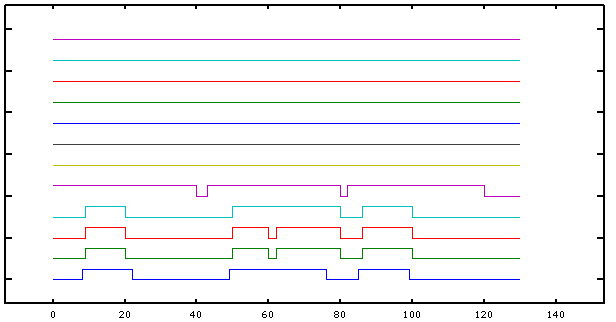
\includegraphics[width=0.9\textwidth]{./testWhiteNoise.png}
 % testWhiteNoise.png: 616x322 pixel, 72dpi, 21.73x11.36 cm, bb=0 0 616 322
\end{figure}
% \subsection{Caso di test di tolleranza al rumore bianco}
% Il protagonista di questo caso di test \`e il file Normal vesicular.wav che contiene un suono respiratorio normale disturbato da un rumore leggero. A questo file aggiungiamo con Audacity del rumore bianco di intensit\`a crescente e valutiamo le prestazioni del sistema. Il file ha le seguenti caratteristiche:
% \begin{itemize}
%  \item 
%     L'intensit\`a massima \`e circa $0.2dB$.
%   \item
%     L'intensit\`a media delle fasi inspiratorie \`e circa $0.08dB$.
%   \item
%     L'intensit\`a media delle fasi di pause respiratorie \`e circa $0.02dB$.
% \end{itemize}
% 
% L'intensit\`a del rumore aggiunto va da $0dB$ a $0.2dB$ con un incremento di $0.02dB$, quindi eseguiamo $11$ test. 
% In nessun caso era presente una apnea troppo lunga e in nessun caso l'algoritmo ha rilevato la presenza di una apnea troppo lunga quindi dal punto di vista del riconoscimento di apnee troppo lunghe, l'algoritmo funziona in modo corretto. 
% \`E comunque interessante valutare l'output dell'algoritmo con un maggior livello di dettaglio. 
% La figura \ref{testNormalWhiteNoise} illustra una rappresentazione dell'output dell'algoritmo sui file di test e contiene un grafico per ogni file di input.
% \begin{figure}
%  \centering
%  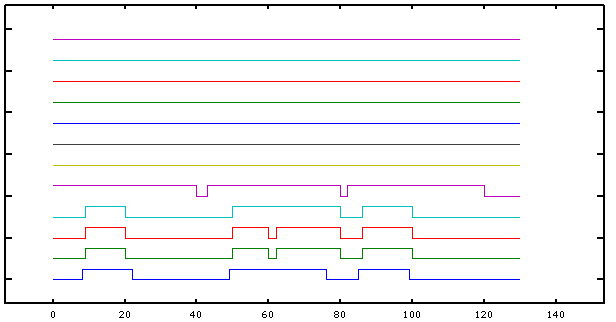
\includegraphics[width=0.9\textwidth]{./testWhiteNoise.png}
%  % testWhiteNoise.png: 1366x768 pixel, 72dpi, 48.19x27.09 cm, bb=0 0 1366 768
%   \caption{Risultati del test di tolleranza al rumore bianco.}
%   \label{testNormalWhiteNoise}
% \end{figure}
% 
% I valori sulle ascisse segnano il tempo in decimi di secondo.
% I grafici contenuti nella figura dal basso verso l'alto escluso il primo sono relativi a file che hanno una quantit\`a di rumore crescente e mostrano quali parti dei rispettivi file vengono riconosciuti come respiro e quali parti vengono riconosciuti come apnea.
% Invece il primo grafico in basso rappresenta il file originale in termini di fasi di respiro e fasi di pausa, stimate da un ascolto del file.
% I valori di questo grafico sono approssimativi e non \`e possibile ottenere valori pi\`u precisi se non si misura il flusso d'aria in modo diretto.
% Notiamo che gli ultimi $7$ grafici dal basso sono semplicemente dei segmenti di retta, questo perch\`e l'algoritmo riconosce l'intero file come respirazione cio\`e non riconosce alcuna pausa. 
% Mentre nei primi $5$ grafici dal basso il segmento di retta pu\`o essere in basso ad indicare una pausa oppure in alto ad indicare la presenza di una inspirazione o di una espirazione.
% 
% 
% % Nel grafico in figura \ref{graficoCasoDiTestRumoreBianco}, l'asse delle ascisse riporta la quantit\`a di rumore bianco aggiunto in termini di percentuale di decibel di rumore rispetto all'intensit\`a massima del respiro, mentre l'asse delle ordinate riporta l'errore calcolato in base a quanto detto nella sottosezione \ref{valutareOutput}.

\end{frame}



